

{Since the least count in the Digital Multimeter is $0.01v$}

{Uncertainty in the measurement of Voltage $ = \pm 0.005v$}

{The Stopping Voltage for the 2nd and 1st order sets of measurements are similar since the intensity of light does not affect the stopping voltage.}

{This supports the Einstein/Planck model of light, according to which the energy of a photon depends on the frequency of light and not its intensity.}


\begin{figure}[H]
	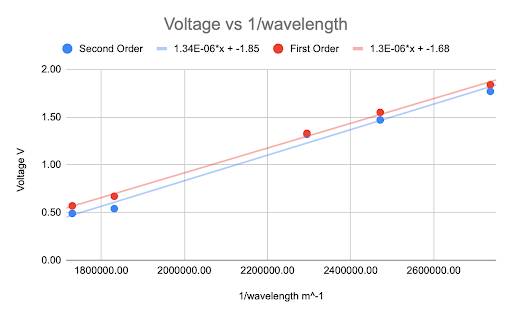
\includegraphics[width=14cm]{vbylambda.png}
\end{figure}

{For the first order,}	
	
	$$\frac{hc}{e} = 1.30\times10^{-6}v$$
	
	$$\frac{\phi}{e} = 1.68v$$
	
	$$\implies h = \frac{1.30\times10^{-6}\times1.6\times10^{-19}}{3\times10^{8}} = 6.93\times10^{-34}Js$$ 
	
	$$\phi = 1.68eV$$
	
{For the second order,}

	$$\frac{hc}{e} = 1.34\times10^{-6}v$$
	
	$$\frac{\phi}{e} = 1.85v$$
	
	$$\implies h = \frac{1.34\times10^{-6}\times1.6\times10^{-19}}{3\times10^{8}} = 7.15\times10^{-34}Js$$
	
	$$\phi = 1.85eV$$
	
{Therfore,}

	$$\frac{\Delta h}{h} = \frac{\Delta \phi}{\phi} = \frac{\Delta V}{V}$$
	
{Considering only the average of all $\frac{\Delta V}{V}$, $\frac{\Delta V}{V} = 0.00519$ for first order and $\frac{\Delta V}{V} = 0.00590$ for second order.}

{$\therefore$ Measured Percentage Error in $h = 0.519\%$ for first order and $h = 0.590\%$ for second order.}

{$\therefore$ Measured Percentage Error in $\phi = 0.519\%$ for first order and $\phi = 0.590\%$ for second order.}

{Absolute Error $\Delta h = 3.60\times10^{-36}Js$ for first order and $\Delta h = 3.71\times10^{-36}Js$.}

{Absolute Error $\Delta \phi = 8.72\times10^{-3}eV$ for first order and $\Delta \phi = 9.60\times10^{-3}eV$.}

{Actual Percentage Error in $h = \frac{h_{i} - h}{h} \times 100$.}

{First Order \% Error $= 4.59\%$.}

{Second Order \% Error $= 7.91\%.}

{The actual errors are more significant than the measured errors. This can be attributed to any human errors made in taking measurements.}


